\section{Kapitel 5: Dynamik}
\begin{tabular}{p{4cm} p{15cm}}
Newton'sche BGL pro Volumeneinheit	& \begin{tabular}[t]{l}
					     $\rho \vec{a} = \vec{F}_{res} = \vec{F}_p + \vec{F}_C + \vec{F}_R$\\
					     $\vec{F}_p = $ Druckgradientenkraft\\
					     $\vec{F}_C = $ Corioliskraft\\
					     $\vec{F}_R = $ Reibungskraft\\
					     $[\vec{F}] = $ N m$^{-3}$
					  \end{tabular}\\
Druckgradientenkraft		& $\boxed{\vec{F}_p = -\vec\nabla p}$\\
Corioliskraft			& \begin{tabular}[t]{p{14cm}}
				    Tr�gheitskraft. Relevant, da wir auf dem beschleunigten (rotierten) Bezugssystem Erde sitzen.\\
				    $\boxed{\vec{F}_C = -\rho f \vec{k} \times \vec{v}}$\\
				    $\quad f = 2\Omega \sin \phi$\\
				    $\qquad \Omega: $ Winkelgeschwindigkeit der Erdrotation\\
				    $\qquad \phi:$ geografische Breite. 0 = �quator, + 90 = Nordpol, -90 = S�dpol\\
				    $\quad\vec{k}:$ Einheitsvektor in z-Rtg.\\
				    $\quad\vec{v}:$ Horizontalgeschwindigkeit eines Luftpakets
				  \end{tabular}\\
geostrophischer Wind		& \begin{tabular}[t]{p{14cm}}
				    Annahme: $\vec{F}_R \ll \vec{F}_C \Rightarrow \vec{F}_C = -\vec{F}_p$\\
				    $\boxed{-\vec\nabla p = \rho f \vec{k} \times \vec{v}_G}$\\
				    Die geostrophische Windrtg. ist immer senkrecht zu $\vec{F}_C$ resp. $\vec{F}_p$, also ist die Windrtg. immer entlang einer Isobare\\
				    $|\vec{v}_G| = \frac{| \vec\nabla p |}{\rho f}$
				  \end{tabular}\\
Kr�ftegleichgewicht mit Reibung	& \begin{tabular}[t]{l}
                               	  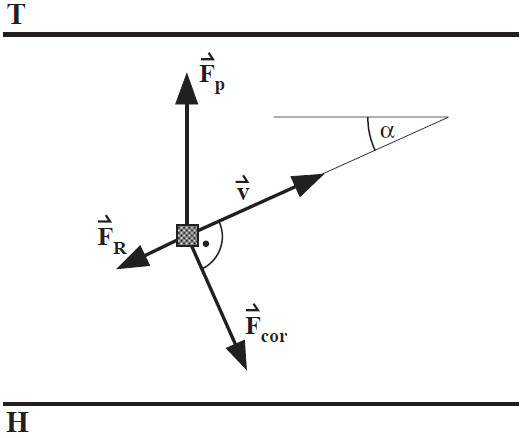
\includegraphics[width = 10cm]{atm_windmitreibung.png}\\
				  $\vec{F}_C \cdot \vec{v} = 0, \vec{F}_R \times \vec{v} = 0, \vec{F}_C + \vec{F}_R = -\vec{F}_P$\\
				  Der Winkel $\alpha$ h�ngt von der Reibung ab.  
                               	  \end{tabular}\\
\end{tabular}
\begin{tabular}{p{4cm} p{15cm}}
Hoch- und Tiefdruckgebiete	& \begin{tabular}[t]{ll}
				    Hoch			& Tief\\
				    relativ station�r		& k�nnen sich schnell bewegen\\
				    schwache Winde		& starke Winde\\
				    Lebensdauer: 3-10 Tage	& Lebensdauer: 1-5 Tage\\
				    Windrtg: $\circlearrowright$& Windrtg: $\circlearrowleft$\\
				  \end{tabular}\\
				& Zeichnung siehe Seite 7 in den Notizen\\
Merkmale einer Front		& \begin{enumerate}
                          	  	\item horiz. Temperaturgradient gross, z.B. 10 \textcelsius auf 100 km
					\item starke �nderung der Windrichtung
					\item aufsteigende Luft $\Rightarrow$ Niederschlag
                          	  \end{enumerate}\\
Polarfrontmodell		& Gem�ss dem klassischen Polarfrontmodell existiert immer eine weltumspannende Polarfront (Druckunterschied zwischen Nord und S�d), sodass sich ein Zyklon gem�ss dem Polarfrontmodell bilden kann (Tiefdruckgebiet entsteht durch St�rung der Front, gem�ss norwegischem Modell)\\
barokline Instabilit�t		& \begin{tabular}[t]{p{14cm}}
				    Tats�chlich ist eine Polarfront nicht immer gegeben, sondern viel schw�chere Druckunterschiede, wobei man von einer baroklinen Zone spricht.\\
				    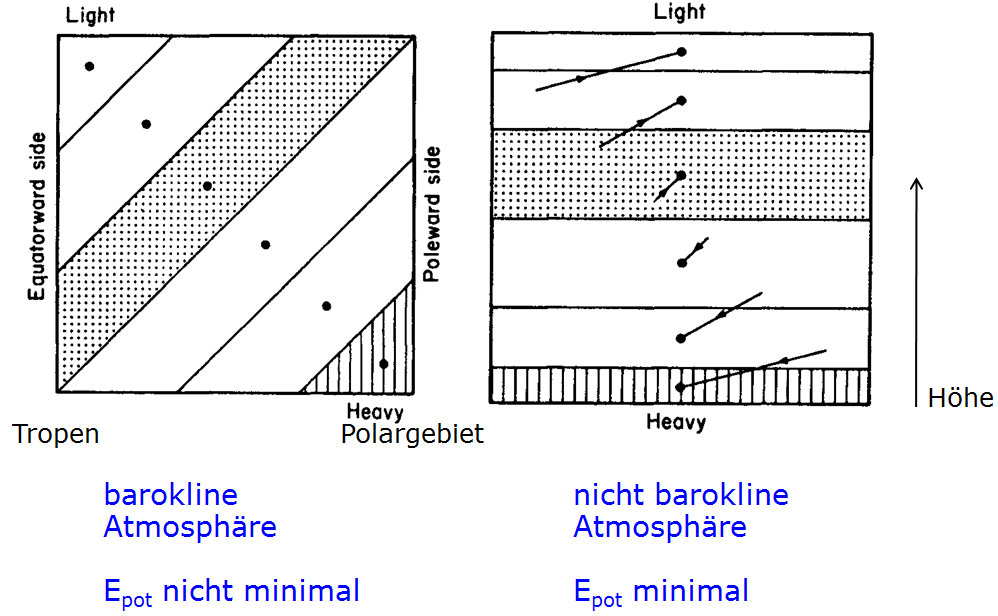
\includegraphics[width=12cm]{atm_baroklineinstabilitaet.png}\\
				    Ideale Extremsituation rechts: $E_{pot}$ ist vollst�ndig minimiert, resp. in $E_{kin}$ (Wind) umgewandelt.\\
				    Ideale Extremsituation links: Die Sonne heizt die Tropen st�rker auf als die Pole. Spezielle Schichtung der Luft. Warme Luft $\Rightarrow$ Leichte Luft\\
				    Eine barokline Zone ist also instabil, somit k�nnen sich Zyklone bilden.
				  \end{tabular}

\end{tabular}